%!TEX root = ../ICR.tex
\chapter{Marco Teórico \label{cap:MarcoTeorico}}

En esta sección se describen las bases teóricas y los conceptos fundamentales que sustentan las dos metodologías de detección de noticias falsas desarrolladas en este proyecto de investigación. Aunque las técnicas son aplicables a diferentes tipos de fraude digital, el enfoque específico se centra en la detección de desinformación periodística. Se abordan desde las técnicas clásicas de representación de texto y optimización metaheurística, hasta los paradigmas de aprendizaje profundo que definen el estado del arte actual.

\section{Detección de Noticias Falsas: Fundamentos y Extensibilidad}
\label{sec:deteccion_noticias_falsas}

La detección de noticias falsas constituye un problema multifacético que requiere un enfoque interdisciplinario, con metodologías que pueden extenderse a otros tipos de fraude digital. La desinformación se caracteriza por ser información deliberadamente falsa o engañosa que se presenta como noticia legítima \cite{bondielli2019survey}. Esta problemática ha evolucionado significativamente con el advenimiento de las redes sociales y los medios digitales, donde la velocidad de propagación supera ampliamente la capacidad de verificación tradicional.

En el contexto de la detección automatizada, se han explorado diferentes enfoques y técnicas. Das et al. \cite{das2022heuristic} propusieron un marco de ensamblaje basado en incertidumbre e impulsado por heurísticas para la detección de noticias falsas en tuits y artículos de noticias. Este enfoque parte de la premisa de que diferentes modelos pueden tener distintas fortalezas y debilidades, y que la combinación inteligente de múltiples predictores puede superar las limitaciones individuales.

El equipo de la Southern Methodist University presentó una solución pionera utilizando procesamiento de lenguaje natural y aprendizaje profundo para analizar tanto titulares como el contenido completo de las noticias \cite{thota2018fake}. Su trabajo estableció un precedente importante al demostrar la viabilidad de la vectorización TF-IDF combinada con redes neuronales densas.

Complementariamente, se ha propuesto un enfoque basado en análisis estilométrico utilizando Procesamiento del Lenguaje Natural (PLN) y Reconocimiento de Entidades Nombradas (NER) para identificar patrones lingüísticos que sugieran baja veracidad de la información \cite{tsai2023stylometric}. Este enfoque aprovecha la hipótesis de que los autores de contenido falso pueden exhibir patrones de escritura distintivos.

\subsection{Impacto Social y Desafíos de la Desinformación}

La rápida propagación de las noticias falsas a través de las redes sociales puede tener graves consecuencias en la sociedad. Como documentan Ali y Zain-Ul-Abdin \cite{ali2020posttruth}, la desinformación puede:

\begin{itemize}
    \item \textbf{Distorsionar la realidad:} Alterando la percepción pública de eventos y hechos
    \item \textbf{Manipular la opinión pública:} Influenciando procesos democráticos y decisiones sociales
    \item \textbf{Incitar a la violencia:} Promoviendo comportamientos agresivos basados en información errónea
    \item \textbf{Difundir propaganda política:} Siendo utilizada como herramienta de influencia partidista
    \item \textbf{Fomentar el odio:} Intensificando divisiones sociales y promoviendo discriminación
    \item \textbf{Provocar pánico:} Especialmente en contextos de crisis sanitarias como la pandemia de COVID-19 \cite{perez2020fake}
\end{itemize}

\subsection{El Problema de las Heurísticas Cognitivas}

La investigación de Ali et al. \cite{ali2021fake} ha demostrado que las heurísticas cognitivas humanas, como la popularidad social (número de ``me gusta'' o compartidos), influyen significativamente en la percepción de credibilidad. Este fenómeno complica la detección, ya que el contenido falso puede volverse viral precisamente por aprovechar estos sesgos cognitivos.

\subsection{Diferenciación Técnica y Transferibilidad: Noticias Falsas vs. Fraude Digital}

Es necesario establecer una distinción técnica clara entre los dominios de aplicación, ya que aunque comparten características computacionales, representan problemas con diferentes objetivos, audiencias y patrones:

\subsubsection{Características Distintivas por Dominio}

\begin{table}[htbp]
\centering
\adjustbox{width=\textwidth,center}{%
\small
\begin{tabular}{|l|l|l|}
\hline
\rowcolor{UAMPurple!20}
\textbf{Aspecto} & \textbf{Noticias Falsas} & \textbf{Fraude Digital} \\
\hline
\textbf{Objetivo primario} & 
\begin{tabular}[t]{@{}l@{}}Manipulación de opinión pública,\\influencia política/social\end{tabular} & 
\begin{tabular}[t]{@{}l@{}}Beneficio económico ilícito,\\acceso no autorizado a recursos\end{tabular} \\
\hline
\textbf{Formato típico} & 
\begin{tabular}[t]{@{}l@{}}Artículos periodísticos,\\imitando medios legítimos\end{tabular} & 
\begin{tabular}[t]{@{}l@{}}Emails de phishing, anuncios\\de inversión, ofertas comerciales\end{tabular} \\
\hline
\textbf{Audiencia objetivo} & 
\begin{tabular}[t]{@{}l@{}}Consumidores de noticias, votantes,\\opinión pública general\end{tabular} & 
\begin{tabular}[t]{@{}l@{}}Potenciales víctimas económicas,\\usuarios con activos digitales\end{tabular} \\
\hline
\textbf{Métrica de éxito} & 
\begin{tabular}[t]{@{}l@{}}Viralidad, alcance,\\influencia en opinión\end{tabular} & 
\begin{tabular}[t]{@{}l@{}}Cantidad de dinero/\\información obtenida\end{tabular} \\
\hline
\textbf{Indicadores lingüísticos} & 
\begin{tabular}[t]{@{}l@{}}Imitación de estilo periodístico,\\fuentes falsas, sensacionalismo político\end{tabular} & 
\begin{tabular}[t]{@{}l@{}}Urgencia económica, ofertas ``limitadas'',\\solicitudes de información personal\end{tabular} \\
\hline
\textbf{Temporalidad} & 
\begin{tabular}[t]{@{}l@{}}Eventos actuales,\\ciclos noticiosos\end{tabular} & 
\begin{tabular}[t]{@{}l@{}}Atemporales, aprovechan\\tendencias económicas\end{tabular} \\
\hline
\end{tabular}
}
\caption{Diferencias técnicas entre dominios de desinformación}
\label{tab:diferencias_dominios}
\end{table}

\subsubsection{Fundamentos de la Transferibilidad Metodológica}

A pesar de sus diferencias conceptuales, ambos dominios comparten características computacionales fundamentales que justifican la transferibilidad de la metodología desarrollada:

\begin{itemize}
    \item \textbf{Naturaleza textual primaria}: Ambos dominios se basan en contenido textual como vector principal de engaño
    \item \textbf{Problema de clasificación binaria}: Se reducen a problemas de clasificación legítimo/malicioso
    \item \textbf{Características estilométricas}: Ambos pueden exhibir patrones lingüísticos distintivos detectables
    \item \textbf{Optimización de hiperparámetros}: Ambos se benefician de técnicas de calibración metaheurística
    \item \textbf{Evaluación mediante métricas estándar}: Utilizan las mismas métricas de clasificación (precisión, recall, F1-Score)
\end{itemize}

\subsubsection{Protocolo de Transferencia Metodológica}

Para aplicar la metodología desarrollada a detección de fraude digital, se requiere el siguiente protocolo de adaptación:

\begin{enumerate}
    \item \textbf{Construcción de corpus específico}: Recopilar y etiquetar datos representativos del tipo de fraude digital objetivo
    \item \textbf{Ajuste de preprocesamiento}: Adaptar técnicas de limpieza según las características del nuevo dominio
    \item \textbf{Re-calibración de hiperparámetros}: Aplicar los mismos algoritmos metaheurísticos pero re-optimizar para el nuevo corpus
    \item \textbf{Incorporación de características específicas}: Añadir características relevantes al nuevo dominio (URLs sospechosas, patrones de solicitud de información)
    \item \textbf{Validación en diferentes dominios}: Evaluar la transferencia utilizando métricas de generalización
\end{enumerate}

\textbf{Enfoque de esta investigación}: Este proyecto desarrolla y valida la metodología en el dominio de noticias falsas en español, estableciendo las bases técnicas para su posterior transferencia a otros tipos de fraude digital. La elección de noticias falsas como dominio inicial se justifica por: (1) disponibilidad de corpus etiquetados, (2) relevancia social en comunidades hispanohablantes, y (3) menor complejidad técnica que permite validar la metodología base antes de extensiones más complejas.

\section{Representación de Texto: Desde TF-IDF hasta Embeddings Contextuales}
\label{sec:representacion_texto}

La evolución de las técnicas de representación textual ha sido fundamental para el progreso en PLN. Esta sección aborda desde los métodos clásicos hasta las representaciones más sofisticadas utilizadas en esta tesis.

\subsection{TF-IDF (Term Frequency-Inverse Document Frequency)}

TF-IDF constituye una de las técnicas más fundamentales y efectivas para la representación de texto. A pesar de su simplicidad conceptual, ha demostrado ser muy efectiva en tareas de clasificación de texto. El proceso implica:

\begin{enumerate}
    \item \textbf{Construcción del vocabulario:} Creación de un diccionario con todas las palabras únicas presentes en el corpus de documentos
    \item \textbf{Cálculo de ponderaciones:} Cada término recibe un peso basado en su frecuencia en el documento (TF) y su rareza en el corpus (IDF)
\end{enumerate}

Aunque este método ignora la gramática y el orden de las palabras, ha demostrado ser efectivo como base para métodos más sofisticados y fue fundamental en los primeros trabajos de clasificación de noticias en español \cite{acosta2019construccion}.

\subsection{Fundamentos Matemáticos de TF-IDF}

TF-IDF introduce ponderación semántica mediante el producto de dos componentes fundamentales:

\begin{equation}
\text{TF-IDF}(t,d,D) = \text{TF}(t,d) \times \text{IDF}(t,D)
\end{equation}

Donde:
\begin{itemize}
    \item \textbf{Frecuencia de Término (TF):} $\text{TF}(t,d) = \frac{f_{t,d}}{\sum_{t' \in d} f_{t',d}}$ - frecuencia relativa del término $t$ en el documento $d$
    \item \textbf{Frecuencia Inversa de Documento (IDF):} $\text{IDF}(t,D) = \log\frac{|D|}{|\{d \in D : t \in d\}|}$ - importancia global del término en la colección
\end{itemize}

Esta ponderación asigna mayor peso a términos que son frecuentes en un documento específico pero raros en el corpus general, mejorando la capacidad discriminativa del modelo \cite{thota2018fake}.

\subsection{Limitaciones de los Métodos Clásicos}

Los enfoques basados en TF-IDF presentan limitaciones fundamentales:
\begin{itemize}
    \item \textbf{Pérdida de información secuencial:} No capturan el orden ni la estructura sintáctica
    \item \textbf{Problema de dispersidad:} Generan representaciones muy dispersas en vocabularios grandes
    \item \textbf{Ausencia de semántica:} No modelan relaciones semánticas entre palabras
    \item \textbf{Falta de contexto:} Una palabra tiene la misma representación independientemente del contexto
\end{itemize}

\section{La Revolución Transformer y los Modelos de Lenguaje Modernos}
\label{sec:transformers_modelos_lenguaje}

\subsection{La Arquitectura Transformer: Fundamentos}

La arquitectura Transformer, introducida por Vaswani et al. \cite{vaswani2017attention} en el trabajo seminal ``Attention Is All You Need'', revolucionó el campo del PLN. Su innovación principal radica en el mecanismo de \textbf{auto-atención (self-attention)}, que permite al modelo calcular representaciones ponderando dinámicamente la importancia de cada elemento en una secuencia con respecto a todos los demás elementos.

\subsubsection{Mecanismo de Atención Multi-Cabeza}

El mecanismo de atención se define matemáticamente como:

\begin{equation}
\text{Attention}(Q,K,V) = \text{softmax}\left(\frac{QK^T}{\sqrt{d_k}}\right)V
\end{equation}

Donde $Q$, $K$, y $V$ representan las matrices de consultas (queries), claves (keys) y valores (values), respectivamente. La atención multi-cabeza extiende este concepto:

\begin{equation}
\text{MultiHead}(Q,K,V) = \text{Concat}(\text{head}_1, ..., \text{head}_h)W^O
\end{equation}

Esta arquitectura permite capturar diferentes tipos de relaciones lingüísticas simultáneamente, superando las limitaciones de los modelos secuenciales previos como RNNs y LSTMs.

\subsection{BERT y la Era del Pre-entrenamiento Bidireccional}

BERT (Bidirectional Encoder Representations from Transformers) \cite{devlin2018bert} introdujo el paradigma de pre-entrenamiento bidireccional, entrenando el modelo para predecir palabras enmascaradas considerando tanto el contexto izquierdo como el derecho. Este enfoque genera representaciones contextuales más ricas que los modelos unidireccionales previos.

\subsubsection{Variantes de BERT para Eficiencia}

El éxito de BERT motivó el desarrollo de variantes más eficientes:
\begin{itemize}
    \item \textbf{DistilBERT} \cite{sanh2019distilbert}: Utiliza destilación de conocimiento para reducir el tamaño del modelo en un 40\% manteniendo el 97\% del rendimiento
    \item \textbf{TinyBERT} \cite{jiao2019tinybert}: Aplica destilación a nivel de transformador y predicción para crear modelos aún más compactos
\end{itemize}

\subsection{Aplicaciones en Detección de Noticias Falsas en Español}

Para el español específicamente, se han desarrollado modelos especializados y evaluaciones:
\begin{itemize}
    \item Martínez-Gallego et al. \cite{martinez2021fake} exploraron la aplicación de BERT y BETO (BERT en español), estableciendo líneas base importantes
    \item Blanco-Fernández et al. \cite{blanco2024enhancing} compararon sistemáticamente BERT y RoBERTa para detección de desinformación política
    \item Shushkevich et al. \cite{shushkevich2023improving} investigaron la mejora de clasificación multiclase usando datos aumentados con ChatGPT
\end{itemize}

\subsection{Grandes Modelos de Lenguaje (LLMs) y Nuevos Paradigmas}

\subsubsection{GPT-3 y el Paradigma Few-Shot}

GPT-3 \cite{brown2020language} marcó un hito al demostrar capacidades emergentes de few-shot learning. Con 175 mil millones de parámetros, mostró que los modelos de gran escala pueden realizar tareas sin ajuste fino específico, solo con ejemplos en el prompt.

\subsubsection{LLaMA y la Democratización de LLMs}

LLaMA \cite{touvron2023llama} representa el esfuerzo por democratizar el acceso a modelos de gran escala, proporcionando alternativas open-source a modelos propietarios. Su arquitectura optimizada permite un rendimiento competitivo con menor costo computacional.

\subsubsection{Modelos Multimodales: Gemini}

Gemini \cite{gemini2023family} introduce capacidades multimodales nativas, procesando texto, imágenes y audio de forma integrada. Esta capacidad es relevante para la detección de desinformación que cada vez más incorpora elementos multimedia.

\subsubsection{IA Constitucional}

El trabajo de Bai et al. \cite{bai2022constitutional} sobre IA Constitucional aborda la alineación y seguridad de los LLMs, estableciendo principios para entrenar modelos más seguros y alineados con valores humanos. Este enfoque es crucial cuando los LLMs se utilizan para tareas de detección de desinformación.

\subsection{El Doble Rol de los LLMs en Detección}

La investigación reciente ha revelado que los LLMs presentan un doble rol:
\begin{itemize}
    \item \textbf{Como ``Buenos Consejeros'':} Pueden ser fine-tuned para detectar noticias falsas con alta precisión \cite{hu2024bad}
    \item \textbf{Como ``Malos Actores'':} Pueden generar desinformación convincente, complicando la detección \cite{su2023fake}
    \item \textbf{Adaptación Necesaria:} Los sistemas de detección deben adaptarse a la era de LLMs \cite{su2023adapting}
\end{itemize}

\section{Optimización Metaheurística en Detección de Fraude}
\label{sec:optimizacion_metaheuristica}

\subsection{Fundamentos de las Metaheurísticas}

Las metaheurísticas son estrategias de optimización de alto nivel que guían procesos de búsqueda para encontrar soluciones de alta calidad en espacios de búsqueda complejos. A diferencia de los algoritmos exactos, las metaheurísticas buscan soluciones ``suficientemente buenas'' en tiempo computacional razonable \cite{anselmo2013diseno}.

\subsubsection{Justificación del Uso de Metaheurísticas en Detección de Noticias Falsas}

La aplicación de metaheurísticas en este dominio se justifica por las siguientes características del problema:

\begin{itemize}
    \item \textbf{Espacio de hiperparámetros complejo:} Los modelos de clasificación (SVM, redes neuronales) tienen múltiples hiperparámetros interdependientes
    \item \textbf{Función objetivo no convexa:} Las métricas de rendimiento (F1-Score, precisión) no son funciones continuas y diferenciables
    \item \textbf{Interacciones no lineales:} Los hiperparámetros interactúan de manera compleja, haciendo ineficaces los métodos de optimización tradicionales
    \item \textbf{Múltiples óptimos locales:} El espacio de búsqueda presenta numerosos máximos locales que pueden atrapar algoritmos determinísticos
    \item \textbf{Eficiencia computacional:} Las metaheurísticas exploran el espacio de forma más inteligente que métodos exhaustivos como grid search
\end{itemize}

\subsubsection{Arquitectura General del Sistema Metaheurístico}

El framework metaheurístico desarrollado sigue una arquitectura modular que permite la intercambiabilidad de algoritmos:

\begin{equation}
\text{Sistema} = \{D, P, A, F, E\}
\end{equation}

Donde:
\begin{itemize}
    \item \textbf{D}: Dataset de noticias preprocesado
    \item \textbf{P}: Pipeline de preprocesamiento (tokenización, TF-IDF)
    \item \textbf{A}: Algoritmo metaheurístico (GA, PSO, SA, VNS, SS)
    \item \textbf{F}: Función objetivo (F1-Score en validación cruzada)
    \item \textbf{E}: Evaluador final en conjunto de prueba
\end{itemize}

\subsubsection{Entradas del Sistema Metaheurístico}

\textbf{1. Datos de Entrada:}
\begin{itemize}
    \item \textbf{Corpus textual:} Noticias en español con etiquetas binarias (REAL/FALSO)
    \item \textbf{División de datos:} 70\% entrenamiento, 10\% validación, 20\% prueba (estratificada)
    \item \textbf{Representación TF-IDF:} Matriz dispersa TF-IDF de dimensión $n \times v$ donde $n$ es el número de documentos y $v$ el tamaño del vocabulario
\end{itemize}

\textbf{2. Espacio de Hiperparámetros:}

Para SVM con kernel RBF:
\begin{align}
C &\in [10^{-3}, 10^{3}] \text{ (parámetro de regularización)} \\
\gamma &\in [10^{-4}, 10^{1}] \text{ (parámetro del kernel RBF)} \\
\text{class\_weight} &\in \{\text{None}, \text{balanced}\} \text{ (balanceado de clases)}
\end{align}

Para TF-IDF:
\begin{align}
\text{max\_features} &\in [1000, 50000] \text{ (tamaño del vocabulario)} \\
\text{min\_df} &\in [1, 10] \text{ (frecuencia mínima de documento)} \\
\text{max\_df} &\in [0.7, 1.0] \text{ (frecuencia máxima de documento)} \\
\text{ngram\_range} &\in \{(1,1), (1,2), (1,3)\} \text{ (rango de n-gramas)}
\end{align}

\subsubsection{Preprocesamiento y Pipeline}

\textbf{Etapa 1: Limpieza Textual}
\begin{enumerate}
    \item \textbf{Normalización de caracteres:} Conversión a minúsculas, eliminación de acentos
    \item \textbf{Filtrado de contenido:} Eliminación de URLs, menciones (@), hashtags
    \item \textbf{Tokenización:} División en tokens usando expresiones regulares
    \item \textbf{Eliminación de stopwords:} Filtrado de palabras vacías en español
    \item \textbf{Validación de longitud:} Exclusión de textos demasiado cortos ($<$ 10 tokens)
\end{enumerate}

\textbf{Etapa 2: Vectorización TF-IDF}
\begin{equation}
\text{TF-IDF}(t,d) = \text{TF}(t,d) \times \log\left(\frac{N}{|\{d' : t \in d'\}|}\right)
\end{equation}

Donde $t$ es un término, $d$ un documento, $N$ el total de documentos, y el denominador cuenta documentos que contienen $t$.

\textbf{Etapa 3: Normalización}
Aplicación de normalización L2 para estabilizar el entrenamiento:
\begin{equation}
\mathbf{x}_{\text{norm}} = \frac{\mathbf{x}}{||\mathbf{x}||_2}
\end{equation}

\subsubsection{Algoritmos Metaheurísticos Implementados}

\textbf{1. Algoritmo Genético (GA)}

\textit{Inspiración biológica:} Evolución natural y selección de especies

\textit{Representación:} Cada individuo es un vector de hiperparámetros codificados
\begin{equation}
\text{Individuo} = [C, \gamma, \text{max\_features}, \text{min\_df}, \text{max\_df}, \text{ngram}]
\end{equation}

\textit{Operadores genéticos:}
\begin{itemize}
    \item \textbf{Selección:} Torneo de tamaño 3
    \item \textbf{Cruce:} Cruce uniforme con probabilidad 0.8
    \item \textbf{Mutación:} Mutación gaussiana con probabilidad 0.1
    \item \textbf{Elitismo:} Preservación del 10\% mejores individuos
\end{itemize}

\textit{Parámetros:}
\begin{align}
\text{Tamaño población} &= 30 \\
\text{Generaciones} &= 50 \\
\text{Tasa cruce} &= 0.8 \\
\text{Tasa mutación} &= 0.1
\end{align}

\textbf{2. Optimización por Enjambre de Partículas (PSO)}

\textit{Inspiración biológica:} Comportamiento de bandadas de aves y cardúmenes

\textit{Ecuaciones de movimiento:}
\begin{align}
v_{i}^{t+1} &= w \cdot v_{i}^{t} + c_1 \cdot r_1 \cdot (p_{i} - x_{i}^{t}) + c_2 \cdot r_2 \cdot (g - x_{i}^{t}) \\
x_{i}^{t+1} &= x_{i}^{t} + v_{i}^{t+1}
\end{align}

Donde:
\begin{itemize}
    \item $v_i^t$: velocidad de la partícula $i$ en iteración $t$
    \item $x_i^t$: posición de la partícula $i$ en iteración $t$
    \item $p_i$: mejor posición personal de la partícula $i$
    \item $g$: mejor posición global del enjambre
    \item $w$: factor de inercia ($w = 0.9$)
    \item $c_1, c_2$: factores de aceleración ($c_1 = c_2 = 2.0$)
    \item $r_1, r_2$: números aleatorios $\in [0,1]$
\end{itemize}

\textit{Parámetros:}
\begin{align}
\text{Tamaño enjambre} &= 30 \\
\text{Iteraciones} &= 50 \\
\text{Factor inercia} &= 0.9 \\
\text{Factores aceleración} &= 2.0
\end{align}

\textbf{3. Recocido Simulado Multi-arranque (MSA)}

\textit{Inspiración física:} Proceso de enfriamiento controlado en metalurgia

\textit{Criterio de aceptación:}
\begin{equation}
P(\text{aceptar}) = \begin{cases}
1 & \text{si } \Delta f \geq 0 \\
e^{\frac{\Delta f}{T}} & \text{si } \Delta f < 0
\end{cases}
\end{equation}

Donde $\Delta f = f(\text{nueva}) - f(\text{actual})$ y $T$ es la temperatura.

\textit{Esquema de enfriamiento:}
\begin{equation}
T_{k+1} = \alpha \cdot T_k, \quad \alpha = 0.95
\end{equation}

\textit{Parámetros:}
\begin{align}
\text{Temperatura inicial} &= 100.0 \\
\text{Temperatura final} &= 0.01 \\
\text{Factor enfriamiento} &= 0.95 \\
\text{Iteraciones por temperatura} &= 10 \\
\text{Número de arranques} &= 5
\end{align}

\textbf{4. Búsqueda en Vecindades Variables (VNS)}

\textit{Principio:} Cambio sistemático de estructuras de vecindad para escapar de óptimos locales

\textit{Estructuras de vecindad:}
\begin{itemize}
    \item $N_1$: Perturbación de un hiperparámetro aleatorio
    \item $N_2$: Perturbación de dos hiperparámetros aleatorios
    \item $N_3$: Perturbación de todos los hiperparámetros
\end{itemize}

\textit{Algoritmo general:}
\begin{enumerate}
    \item Inicializar solución $x$
    \item Para cada vecindad $k = 1, 2, 3$:
    \item \quad Generar $x'$ en $N_k(x)$
    \item \quad Aplicar búsqueda local desde $x'$ → $x''$
    \item \quad Si $f(x'') > f(x)$: $x = x''$, $k = 1$
    \item \quad Sino: $k = k + 1$
    \item Repetir hasta criterio de parada
\end{enumerate}

\textbf{5. Búsqueda Dispersa (SS)}

\textit{Principio:} Combinar soluciones de calidad y diversas para generar nuevas soluciones

\textit{Componentes principales:}
\begin{itemize}
    \item \textbf{Conjunto de referencia:} 10 soluciones (5 de calidad + 5 diversas)
    \item \textbf{Generación de subconjuntos:} Todas las combinaciones de tamaño 2
    \item \textbf{Método de combinación:} Promedio ponderado por fitness
    \item \textbf{Mejora:} Búsqueda local en nuevas soluciones
    \item \textbf{Actualización:} Reemplazo de peores soluciones
\end{itemize}

\subsubsection{Función Objetivo y Evaluación}

\textbf{Función objetivo principal:}
\begin{equation}
f(\theta) = \text{F1-Score}_{CV}(\theta)
\end{equation}

Donde $\theta$ representa el vector de hiperparámetros y $\text{F1-Score}_{CV}$ es el F1-Score promedio en validación cruzada estratificada de 5 pliegues.

\textbf{Métricas de evaluación secundarias:}
\begin{align}
\text{Precisión} &= \frac{TP}{TP + FP} \\
\text{Recall} &= \frac{TP}{TP + FN} \\
\text{F1-Score} &= \frac{2 \times \text{Precisión} \times \text{Recall}}{\text{Precisión} + \text{Recall}} \\
\text{Exactitud} &= \frac{TP + TN}{TP + TN + FP + FN}
\end{align}

\subsubsection{Etapas del Proceso Metaheurístico}

\textbf{Etapa 1: Inicialización}
\begin{enumerate}
    \item Cargar y dividir el dataset
    \item Definir espacios de búsqueda para hiperparámetros
    \item Inicializar población/enjambre según el algoritmo
    \item Configurar parámetros del algoritmo metaheurístico
\end{enumerate}

\textbf{Etapa 2: Evaluación de Fitness}
\begin{enumerate}
    \item Para cada configuración de hiperparámetros:
    \item \quad Construir pipeline TF-IDF + SVM
    \item \quad Entrenar en conjunto de entrenamiento
    \item \quad Evaluar en validación cruzada 5-fold
    \item \quad Calcular F1-Score promedio como fitness
\end{enumerate}

\textbf{Etapa 3: Evolución/Optimización}
\begin{enumerate}
    \item Aplicar operadores específicos del algoritmo
    \item Generar nuevas configuraciones candidatas
    \item Evaluar fitness de nuevas configuraciones
    \item Actualizar población/enjambre según criterios del algoritmo
    \item Verificar criterios de convergencia
\end{enumerate}

\textbf{Etapa 4: Selección Final}
\begin{enumerate}
    \item Identificar la mejor configuración encontrada
    \item Re-entrenar modelo con configuración óptima
    \item Evaluar en conjunto de prueba independiente
    \item Reportar métricas finales
\end{enumerate}

\subsubsection{Salidas del Sistema Metaheurístico}

\textbf{1. Configuración Óptima de Hiperparámetros:}
\begin{itemize}
    \item Valores óptimos para cada hiperparámetro del modelo
    \item Historia de convergencia del algoritmo
    \item Número de evaluaciones realizadas
    \item Tiempo total de optimización
\end{itemize}

\textbf{2. Modelo Entrenado Optimizado:}
\begin{itemize}
    \item Vectorizador TF-IDF configurado
    \item Clasificador SVM entrenado
    \item Pipeline completo listo para predicción
\end{itemize}

\textbf{3. Métricas de Rendimiento:}
\begin{itemize}
    \item F1-Score, Precisión, Recall, Exactitud en conjunto de prueba
    \item Matriz de confusión
    \item Curvas de convergencia
    \item Análisis de importancia de hiperparámetros
\end{itemize}

\textbf{4. Análisis Comparativo:}
\begin{itemize}
    \item Comparación entre algoritmos metaheurísticos
    \item Análisis de eficiencia computacional
    \item Estudio de robustez y estabilidad
\end{itemize}

En el contexto de la detección de noticias falsas, las metaheurísticas abordan varios problemas de optimización, con metodologías transferibles a otros tipos de fraude digital:
\begin{itemize}
    \item \textbf{Calibración de hiperparámetros:} Optimización de parámetros de modelos de ML/DL
    \item \textbf{Selección de características:} Identificación de subconjuntos óptimos de variables
    \item \textbf{Arquitectura neural:} Diseño automático de topologías de red
    \item \textbf{Balanceado de datos:} Optimización de técnicas de muestreo
\end{itemize}

\subsubsection{Comparación de Algoritmos Metaheurísticos}

La Tabla \ref{tab:comparacion_metaheuristicas} presenta una comparación sistemática de los cinco algoritmos implementados, destacando sus características distintivas, ventajas y limitaciones en el contexto de optimización de hiperparámetros para detección de noticias falsas.

\begin{table}[htbp]
\centering
\adjustbox{width=\textwidth,center}{%
\small
\begin{tabular}{|l|l|l|l|l|}
\hline
\rowcolor{UAMPurple!20}
\textbf{Algoritmo} & \textbf{Inspiración} & \textbf{Fortalezas} & \textbf{Limitaciones} & \textbf{Parámetros Clave} \\
\hline
\textbf{GA} & Evolución biológica & 
\begin{tabular}[t]{@{}l@{}}Exploración global robusta\\Paralelización natural\\Buena diversidad poblacional\end{tabular} & 
\begin{tabular}[t]{@{}l@{}}Convergencia lenta\\Muchos parámetros a ajustar\\Puede estancarse prematuramente\end{tabular} & 
\begin{tabular}[t]{@{}l@{}}Población: 30\\Generaciones: 50\\Cruce: 0.8\\Mutación: 0.1\end{tabular} \\
\hline
\textbf{PSO} & 
\begin{tabular}[t]{@{}l@{}}Comportamiento\\de enjambre\end{tabular} & 
\begin{tabular}[t]{@{}l@{}}Convergencia rápida\\Pocos parámetros\\Fácil implementación\end{tabular} & 
\begin{tabular}[t]{@{}l@{}}Puede convergir prematuramente\\Sensible a parámetros\\Exploración limitada\end{tabular} & 
\begin{tabular}[t]{@{}l@{}}Partículas: 30\\Iteraciones: 50\\Inercia: 0.9\\Aceleración: 2.0\end{tabular} \\
\hline
\textbf{SA/MSA} & 
\begin{tabular}[t]{@{}l@{}}Recocido\\de metales\end{tabular} & 
\begin{tabular}[t]{@{}l@{}}Escape de óptimos locales\\Base teórica sólida\\Múltiples arranques\end{tabular} & 
\begin{tabular}[t]{@{}l@{}}Esquema de enfriamiento crítico\\Búsqueda individual\\Muchas evaluaciones\end{tabular} & 
\begin{tabular}[t]{@{}l@{}}T inicial: 100\\T final: 0.01\\Enfriamiento: 0.95\\Arranques: 5\end{tabular} \\
\hline
\textbf{VNS} & 
\begin{tabular}[t]{@{}l@{}}Cambio sistemático\\de vecindades\end{tabular} & 
\begin{tabular}[t]{@{}l@{}}Escape sistemático de óptimos\\Combinación exploración/explotación\\Flexibilidad en vecindades\end{tabular} & 
\begin{tabular}[t]{@{}l@{}}Dependiente de definición de vecindades\\Puede ser costoso computacionalmente\\Diseño específico del problema\end{tabular} & 
\begin{tabular}[t]{@{}l@{}}Vecindades: 3\\Iteraciones: 100\\Búsqueda local: Hill climbing\end{tabular} \\
\hline
\textbf{SS} & 
\begin{tabular}[t]{@{}l@{}}Combinación de\\soluciones de calidad\end{tabular} & 
\begin{tabular}[t]{@{}l@{}}Balance calidad-diversidad\\Intensificación y diversificación\\Memoria adaptativa\end{tabular} & 
\begin{tabular}[t]{@{}l@{}}Complejo de implementar\\Muchos componentes\\Sensible a tamaño de referencia\end{tabular} & 
\begin{tabular}[t]{@{}l@{}}Ref. Set: 10\\Combinaciones: todas\\Mejora: local search\\Actualizaciones: dinámicas\end{tabular} \\
\hline
\end{tabular}
}
\caption{Comparación de algoritmos metaheurísticos implementados}
\label{tab:comparacion_metaheuristicas}
\end{table}

\subsubsection{Criterios de Selección y Justificación}

La selección de estos cinco algoritmos metaheurísticos se basó en criterios específicos de idoneidad para el problema de optimización de hiperparámetros en detección de noticias falsas:

\begin{enumerate}
    \item \textbf{Diversidad de paradigmas:} Se incluyeron representantes de las principales familias de metaheurísticas (evolutivas, de enjambre, basadas en trayectoria, de memoria)
    
    \item \textbf{Eficiencia computacional:} Algoritmos con balance adecuado entre calidad de solución y tiempo de cómputo
    
    \item \textbf{Robustez empírica:} Métodos con evidencia documentada de efectividad en problemas de optimización de ML
    
    \item \textbf{Implementación práctica:} Algoritmos con parámetros bien establecidos y implementaciones estables
    
    \item \textbf{Complementariedad:} Enfoques que exploran el espacio de búsqueda de maneras fundamentalmente diferentes
\end{enumerate}

Esta selección permite una evaluación comprehensiva de diferentes estrategias de optimización, proporcionando insights sobre qué características algorítmicas son más efectivas para el problema específico de calibración de detectores de noticias falsas.

\subsubsection{Justificación Frente a Métodos Alternativos}

\textbf{Comparación con Grid Search:}
\begin{itemize}
    \item \textbf{Eficiencia:} Grid search requiere $O(n^k)$ evaluaciones donde $n$ es el número de valores por parámetro y $k$ el número de parámetros. Para este problema: $10^6$ evaluaciones vs. 1,500 de metaheurísticas
    \item \textbf{Escalabilidad:} Grid search se vuelve impracticable con espacios de alta dimensión
    \item \textbf{Optimización continua:} Las metaheurísticas manejan parámetros continuos naturalmente
\end{itemize}

\textbf{Comparación con Random Search:}
\begin{itemize}
    \item \textbf{Inteligencia dirigida:} Las metaheurísticas aprenden del histórico de evaluaciones
    \item \textbf{Convergencia:} Random search no garantiza convergencia hacia regiones prometedoras
    \item \textbf{Explotación vs. Exploración:} Las metaheurísticas balancean sistemáticamente ambos aspectos
\end{itemize}

\textbf{Comparación con Optimización Bayesiana:}
\begin{itemize}
    \item \textbf{Asunciones del modelo:} Bayesian optimization asume suavidad que puede no cumplirse en métricas de ML
    \item \textbf{Costo computacional:} El cálculo de la función de adquisición puede ser costoso
    \item \textbf{Flexibilidad:} Las metaheurísticas son más flexibles para restricciones complejas
\end{itemize}

\textbf{Comparación con Gradient-based Methods:}
\begin{itemize}
    \item \textbf{Diferenciabilidad:} Las métricas de clasificación (F1-Score) no son diferenciables
    \item \textbf{Naturaleza discreta:} Algunos hiperparámetros son categóricos o discretos
    \item \textbf{Robustez:} Los métodos basados en gradiente son sensibles a óptimos locales
\end{itemize}

\subsubsection{Flujo del Proceso Metaheurístico}

La Figura \ref{fig:flujo_metaheuristicas} ilustra el flujo completo del proceso de optimización metaheurística aplicado a la detección de noticias falsas, desde la entrada de datos hasta la obtención del modelo optimizado final.

\begin{figure}[h!]
    \centering
    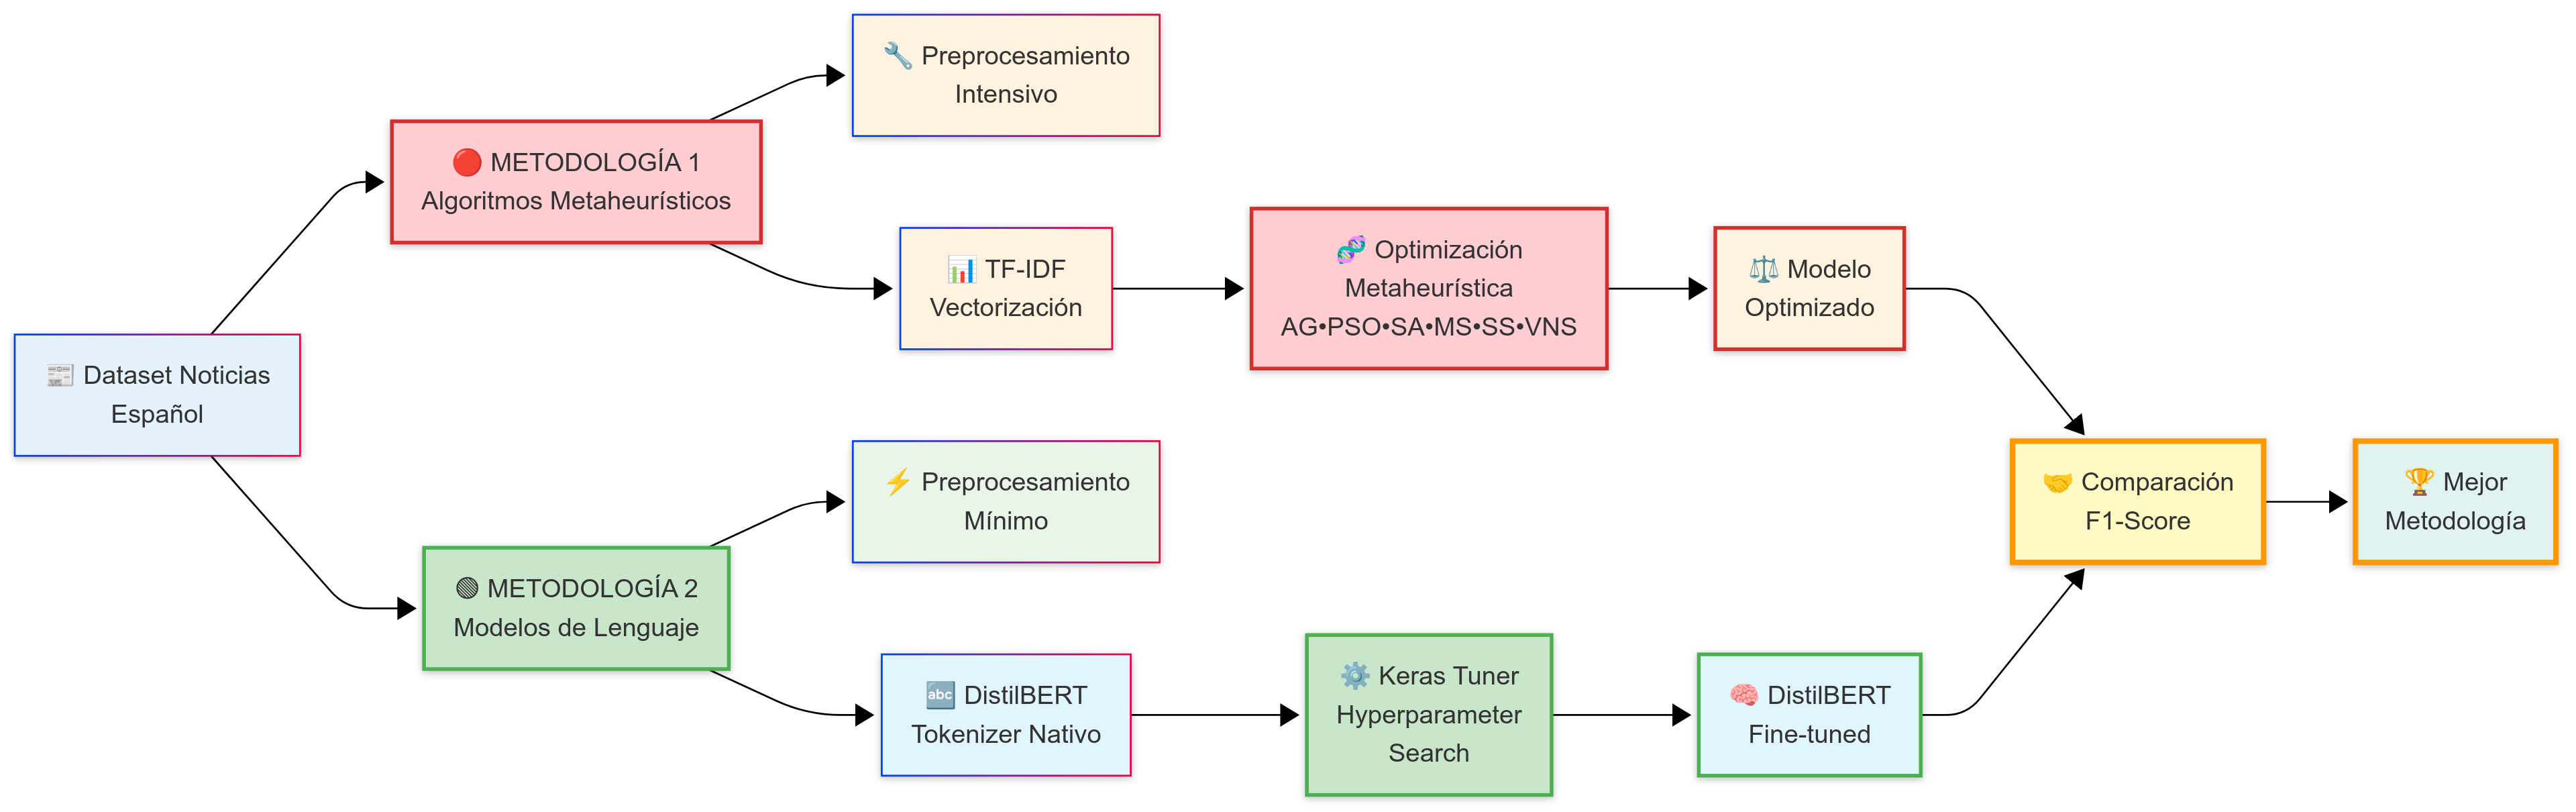
\includegraphics[width=\textwidth]{Imagenes/figura2Flujo.png}
    \caption{Flujo del proceso de optimización metaheurística para detección de noticias falsas. Se muestra la transformación desde datos textuales hasta el modelo optimizado final, pasando por las etapas de preprocesamiento, optimización y evaluación.}
    \label{fig:flujo_metaheuristicas}
\end{figure}

Este flujo garantiza:
\begin{itemize}
    \item \textbf{Reproducibilidad:} Cada etapa está claramente definida con parámetros específicos
    \item \textbf{Escalabilidad:} El proceso puede aplicarse a corpus de diferentes tamaños
    \item \textbf{Transferibilidad:} La metodología es aplicable a otros problemas de clasificación textual
    \item \textbf{Transparencia:} Cada decisión algorítmica está justificada y documentada
\end{itemize}

\subsubsection{Consideraciones de Implementación}

\textbf{Manejo de Memoria:}
\begin{itemize}
    \item Uso de matrices dispersas (scipy.sparse) para representaciones TF-IDF
    \item Liberación explícita de memoria entre evaluaciones
    \item Procesamiento por lotes para corpus grandes
\end{itemize}

\textbf{Paralelización:}
\begin{itemize}
    \item Evaluación paralela de individuos en GA
    \item Vectorización de operaciones en PSO
    \item Múltiples arranques independientes en SA
\end{itemize}

\textbf{Validación y Robustez:}
\begin{itemize}
    \item Validación cruzada estratificada para preservar distribución de clases
    \item Múltiples ejecuciones independientes para análisis estadístico
    \item Manejo de casos extremos y configuraciones inválidas
\end{itemize}

\subsubsection{Métricas de Monitoreo del Proceso}

Durante la ejecución de cada algoritmo metaheurístico, se monitorizan las siguientes métricas:

\begin{enumerate}
    \item \textbf{Convergencia:} Evolución del mejor fitness a lo largo de las iteraciones
    \item \textbf{Diversidad:} Medida de dispersión en la población/enjambre
    \item \textbf{Estagnación:} Número de iteraciones sin mejora significativa
    \item \textbf{Eficiencia:} Número de evaluaciones para alcanzar convergencia
    \item \textbf{Estabilidad:} Variabilidad entre ejecuciones independientes
\end{enumerate}

Estas métricas permiten:
\begin{itemize}
    \item Ajustar parámetros de los algoritmos dinámicamente
    \item Detectar convergencia prematura o estagnación
    \item Comparar objetivamente el rendimiento de diferentes metaheurísticas
    \item Identificar configuraciones problemáticas o excepcionales
\end{itemize}

\subsection{Aplicaciones en Detección de Noticias Falsas}

\subsubsection{Modelado como Problema de Scheduling}

Aqil y Lahby \cite{aqil2021modeling} propusieron una perspectiva innovadora, modelando la detección de noticias falsas como un problema de Job Shop Scheduling. Compararon tres metaheurísticas:
\begin{itemize}
    \item \textbf{Algoritmo Genético (GA):} Evolución de soluciones mediante selección, cruce y mutación
    \item \textbf{Optimización por Enjambre de Partículas (PSO):} Búsqueda inspirada en comportamiento de bandadas
    \item \textbf{Colonia de Abejas Artificiales (ABC):} Algoritmo basado en comportamiento de forrajeo de abejas
\end{itemize}

Sus resultados mostraron que el algoritmo Iterated Greedy (IG) superó a las metaheurísticas bioinspiradas en este contexto específico.

\subsubsection{Optimización de Hiperparámetros en Deep Learning}

Bacanin et al. \cite{bacanin2023benefits} demostraron los beneficios de usar metaheurísticas para la calibración de hiperparámetros en modelos de deep learning. Su investigación mostró mejoras significativas sobre métodos tradicionales como grid search y random search:

\begin{itemize}
    \item \textbf{Eficiencia computacional:} Exploración más inteligente del espacio de hiperparámetros
    \item \textbf{Evitación de óptimos locales:} Capacidad de escape de configuraciones subóptimas
    \item \textbf{Adaptabilidad:} Ajuste dinámico según el comportamiento del modelo
\end{itemize}

La investigación que publiqué en \cite{hurtado2024calibracion} específicamente aborda la calibración de hiperparámetros en algoritmos metaheurísticos para detección de noticias falsas (como caso específico de fraude digital), proporcionando un marco metodológico relevante para esta tesis.

\subsubsection{Frameworks de Ensemble Heurístico}

Das et al. \cite{das2022heuristic} desarrollaron un marco de ensemble que combina:
\begin{itemize}
    \item \textbf{Modelos pre-entrenados:} BERT y similares para captura semántica
    \item \textbf{Características estadísticas:} Metadatos como URL, autor, timestamp
    \item \textbf{Heurísticas de incertidumbre:} Medidas de confianza para ponderación de predictores
\end{itemize}

Este enfoque híbrido logró F1-scores superiores al 95% en conjuntos de datos de referencia.

\subsection{Metaheurísticas para Detección de Fraude Financiero}

\subsubsection{Optimización Multi-objetivo}

Hidayattullah et al. \cite{hidayattullah2020financial} aplicaron metaheurísticas para optimizar la detección de fraude en estados financieros. Su enfoque multi-objetivo consideró:
\begin{itemize}
    \item \textbf{Precisión de clasificación:} Maximización de métricas de rendimiento
    \item \textbf{Eficiencia computacional:} Minimización de tiempo de entrenamiento
    \item \textbf{Robustez:} Estabilidad ante variaciones en los datos
\end{itemize}

Los resultados mostraron que SVM optimizado con Algoritmo Genético alcanzó 96.15\% de precisión, superando significativamente a métodos tradicionales.

\subsubsection{Optimización de Procesos Gaussianos}

Horak y Sabek \cite{horak2023gaussian} exploraron la optimización de hiperparámetros en Gaussian Process Regression para predicción de dificultades financieras. Su trabajo destaca la importancia de la calibración metaheurística en modelos probabilísticos.

\subsection{Algoritmos Híbridos Modernos}

\subsubsection{Enfoques Multi-thread}

Yildirim \cite{yildirim2023novel} propuso un enfoque metaheurístico híbrido multi-thread que optimiza simultáneamente:
\begin{itemize}
    \item Selección de características
    \item Parámetros del algoritmo de clasificación
    \item Arquitectura del ensemble
\end{itemize}

\subsubsection{PSO Adaptativo}

Deshai y Bhaskara Rao \cite{deshai2023unmasking} desarrollaron un enfoque CNN con PSO adaptativo para detectar reseñas falsas online. Su algoritmo PSO adaptativo ajusta dinámicamente los parámetros de velocidad e inercia basándose en el rendimiento de la iteración actual.

\section{Integración de Enfoques: Hacia Sistemas Híbridos}
\label{sec:integracion_enfoques}

\subsection{Combinación de Representaciones Clásicas y Modernas}

La tendencia actual en detección de noticias falsas favorece sistemas híbridos que combinan (principios aplicables a otros tipos de fraude digital):
\begin{itemize}
    \item \textbf{Características lingüísticas tradicionales:} TF-IDF, n-gramas, métricas de legibilidad
    \item \textbf{Embeddings contextuales:} Representaciones de BERT y similares
    \item \textbf{Metadatos estructurales:} Información temporal, de red social, y fuente
    \item \textbf{Características estilométricas:} Patrones de puntuación, longitud de oraciones, complejidad sintáctica
\end{itemize}

\subsection{Arquitecturas de Ensemble Optimizadas}

Las arquitecturas modernas emplean:
\begin{itemize}
    \item \textbf{Ensemble de modelos heterogéneos:} Combinación de clasificadores tradicionales y deep learning
    \item \textbf{Ponderación adaptativa:} Pesos dinámicos basados en confianza y rendimiento
    \item \textbf{Fusión de decisiones:} Estrategias sofisticadas para combinar predicciones múltiples
\end{itemize}

\subsection{Optimización End-to-End}

Zhang et al. \cite{zhang2023using} exploraron el uso de LLMs para optimización de hiperparámetros, abriendo nuevas posibilidades para la optimización automática de pipelines completos de detección.

\section{Desafíos y Direcciones Futuras}
\label{sec:desafios_direcciones}

\subsection{Desafíos Técnicos}

\begin{itemize}
    \item \textbf{Adaptación multilingüe:} Desarrollo de modelos robustos para múltiples idiomas
    \item \textbf{Detección en tiempo real:} Optimización para procesamiento de streams de alta velocidad
    \item \textbf{Robustez adversarial:} Resistencia a ataques de evasión sofisticados
    \item \textbf{Explicabilidad:} Desarrollo de modelos interpretables para decisiones críticas
\end{itemize}

\subsection{Consideraciones Éticas y Sociales}

\begin{itemize}
    \item \textbf{Sesgos algorítmicos:} Mitigación de discriminación en sistemas de detección
    \item \textbf{Privacidad:} Protección de datos personales en análisis de contenido
    \item \textbf{Transparencia:} Apertura en metodologías y criterios de detección
    \item \textbf{Impacto social:} Consideración de efectos en libertad de expresión y democracia
\end{itemize}

\section{Síntesis del Marco Teórico}
\label{sec:sintesis_marco}

Este marco teórico establece los fundamentos para las dos metodologías desarrolladas en esta tesis:

\begin{enumerate}
    \item \textbf{Enfoque Clásico Optimizado:} Utiliza representaciones TF-IDF con optimización metaheurística de hiperparámetros, proporcionando una línea base sólida y computacionalmente eficiente
    
    \item \textbf{Enfoque de Deep Learning:} Emplea modelos Transformer pre-entrenados con fine-tuning, aprovechando representaciones contextuales sofisticadas
\end{enumerate}

La combinación de ambos enfoques, sustentada en la literatura revisada, permite abordar el problema de detección de noticias falsas desde múltiples perspectivas, maximizando tanto la efectividad como la eficiencia computacional del sistema propuesto. La metodología desarrollada establece principios transferibles para abordar otros tipos de fraude digital con las adaptaciones correspondientes.

El marco establece también la base teórica para la contribución metodológica principal de esta tesis: la aplicación sistemática de técnicas metaheurísticas para la optimización de hiperparámetros en ambos paradigmas, desde clasificadores tradicionales hasta modelos de deep learning, en el contexto específico de textos en español.